\chapter{Simulations of a Plenoptic 1.0 System}
\markboth{\MakeUppercase{Simulations of a Plenoptic 1.0 System}}{}
\label{chap:chapter4}
\section{Introduction}
\label{sec:intro3}
The main purpose of the work described in this chapter is to prove that the images obtained simulating a plenoptic imaging system using the wave simulation toolbox described in chapter \ref{chap:fresnel} are equivalent to the ones obtained with conventional ray tracing techniques. In addition to that the effects of diffraction will be explained and evaluated. Simulations were run also to better understand the existing rendering algorithms, the synthetic refocusing algorithm and depth estimation. These algorithms based on ray optics give the expected results on the raw images produced using the wave optics simulation toolbox.
The methods used to design, develop and test the data processing algorithms, such as rendering, synthetic refocus and depth estimation algorithms from the digitally generated light fields data are described. All the light field processing algorithms presented in this chapter use the third parametrization of the light field described in section \ref{sec:LFparam} that is the four dimensional representation of the intensity recorded on the sensor. Each point of this four dimensional array is a ray at the position \textit{x} and \textit{y} with a direction $\theta_x$ and $\theta_y$ \cite{ng2006digital,georgiev2010focused}.
\section{Description of the System}
\label{sec:system10}
The plenoptic 1.0 camera described in section \ref{sec:camera10} has been modelled as a 2f system composed of a main lens, a micro lens array and a sensor as shown in figure \ref{fig:pleno10_system}. The micro lens array is placed at a distance \textit{z=2f} from the main lens, where \textit{f} is the focal length of the main lens, and the sensor is placed at a distance $f_\mu$ from the micro array plane that is also the focal length of the lenslets. In this configuration the lenslet array plane is conjugated with the object plane, while the sensor plane is conjugated with the main lens plane. In order to satisfy the f-number matching condition described in section \ref{sec:camera10} the software automatically sets the aperture of the main lens according to the propagation distances, the micro lens array parameters, the resolution \textit{N} of the input field, the wavelength of the light used and the micro array parameters settings. 
\begin{figure}[H]
	\centering
	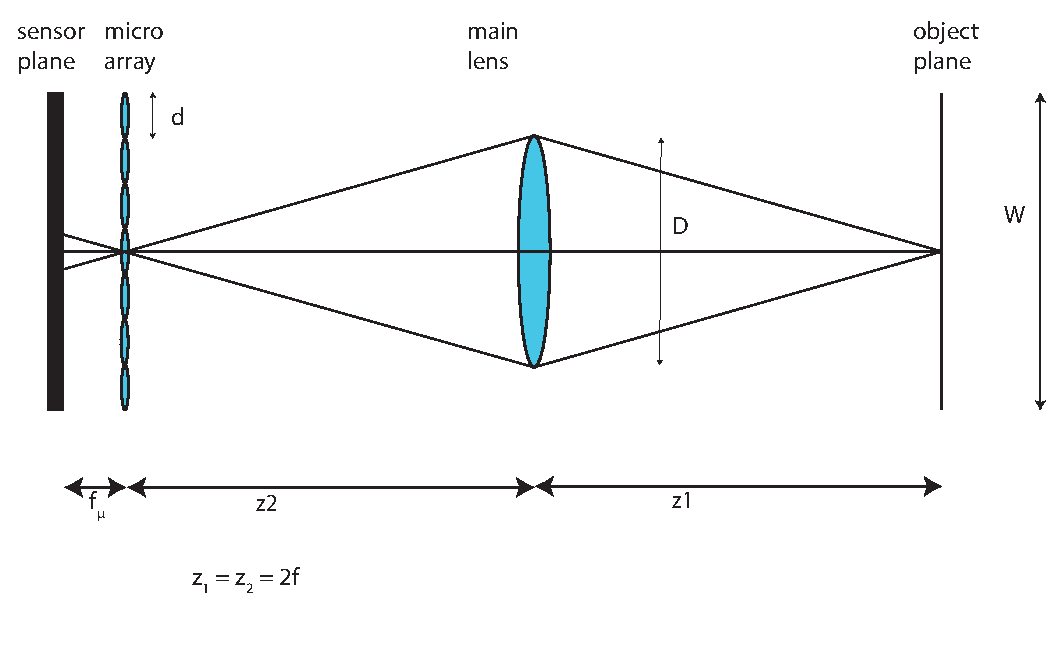
\includegraphics[width=.7\textwidth]{C:/Users/Massimo/Documents/Thesis/Thesis_PhD/plenoptic101.eps}
	\caption{\label{fig:pleno10_system} Parameters that characterize the micro lens array are: the pitch $p$, defined as the distance between the centres of two lenslets, the diameter d, the number of lenslets per row N and the size of the micro array W. }
\end{figure}
The micro array parameters are illustrated in figure \ref{fig:microarray1} and are the pitch, the diameter of the single lenslet, the number of lenslet in a row and the size of the array. In all simulations the pitch of the lenslets is equal to the diameter and the lenslets are arranged in a square matrix. 
\begin{figure}[H]
	\centering
	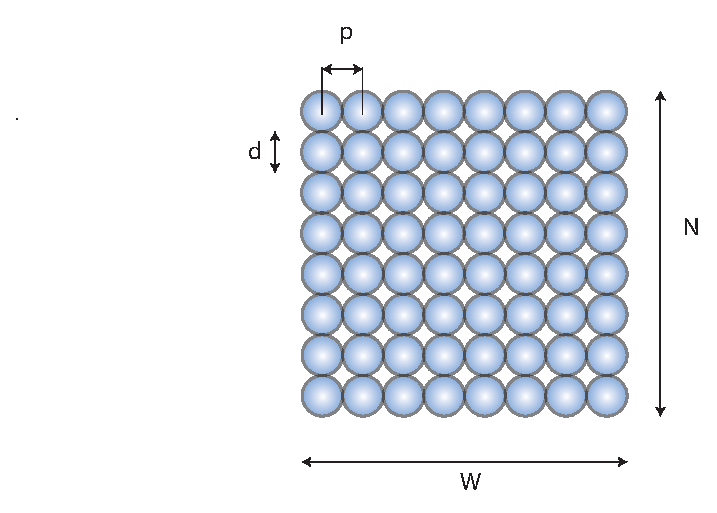
\includegraphics[width=.7\textwidth]{C:/Users/Massimo/Documents/Thesis/Thesis_PhD/micro_array.eps}
	\caption{\label{fig:microarray1} Parameters that characterize the micro lens array. }
\end{figure}
\subsection{Diffraction Effects on the System}
\label{sec:diffraction}
Diffraction from the lenslet's circular aperture can generate cross talk between neighbouring sub images since the light form a single lenslet falls in the sub image of the neighbouring lenslet. Because of this, blur is present in the rendered image resulting in a loss of spatial resolution. To avoid this loss of resolution the diameter of each lenslet should be large enough so that the diameter of the Airy disk is smaller than the lenslet diameter. As seen in equation \ref{eq:airy} for a lens with a circular aperture, the diameter of the Airy disk at its focal plane is
\begin{equation}
\label{eq:airy1}
d_{Airy} = 2.44\lambda z/d
\end{equation}
 In order to avoid diffraction induced cross talk the lenslet diameter should be:
\begin{equation}
\label{eq:lenscond}
D>2.44 \dfrac{\lambda z}{D}
\end{equation} 
Therefore the condition of \textit{D} is:
\begin{equation}
\label{eq:min_diam}
D>\sqrt{2.44\lambda f_{\mu}}
\end{equation}
This is a very important result and it is an original contribution to the field, since it represents the first design condition ever evaluated form diffraction considerations. 
Therefore when choosing or designing a lenslet array for plenoptic imaging the lenslet diameter and the focal length should satisfy equation \ref{eq:min_diam}. The acceptable values belong to the area above the blue line in the diagram shown in figure \ref{fig:mindiam}.
\begin{figure}[H]
	\centering
	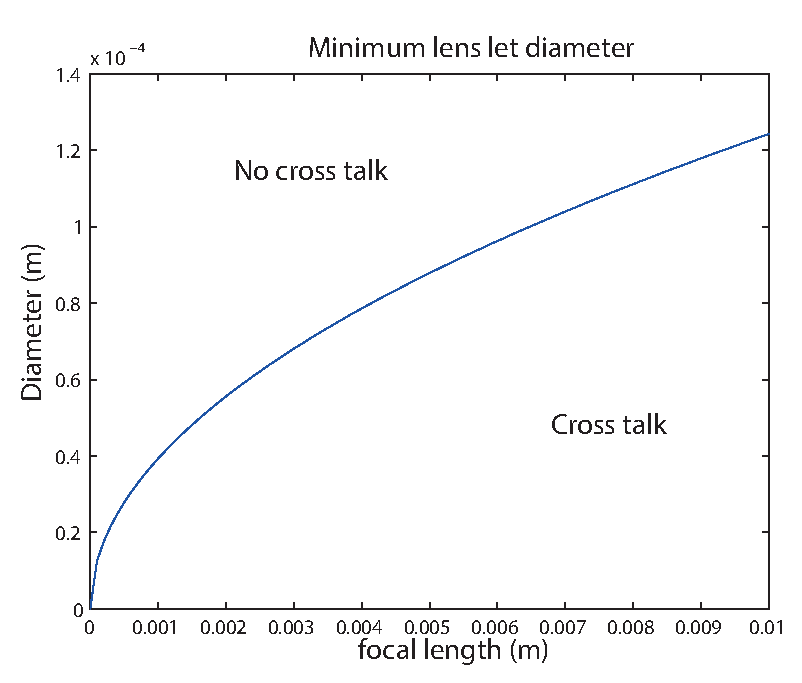
\includegraphics[width=.7\textwidth]{C:/Users/Massimo/Documents/Thesis/Thesis_PhD/mindiameter.eps}
	\caption{\label{fig:mindiam} Values of acceptable lenslet diameter to avoid diffraction induced cross talk. }
\end{figure}
The effect of cross talk between lenslets on the raw image is shown in figure \ref{fig:crosstalk1}.
This image was obtained simulating a point source imaged by a 120 mm lens placed in a 2f configuration with the lens let array. The sensor resolution was 2000 by 2000 pixels and the micro array was made of 101 by 101 lenslets with a diameter of 100 $\mu$m and a focal length of 100 mm.
\begin{figure}[H]
	\centering
	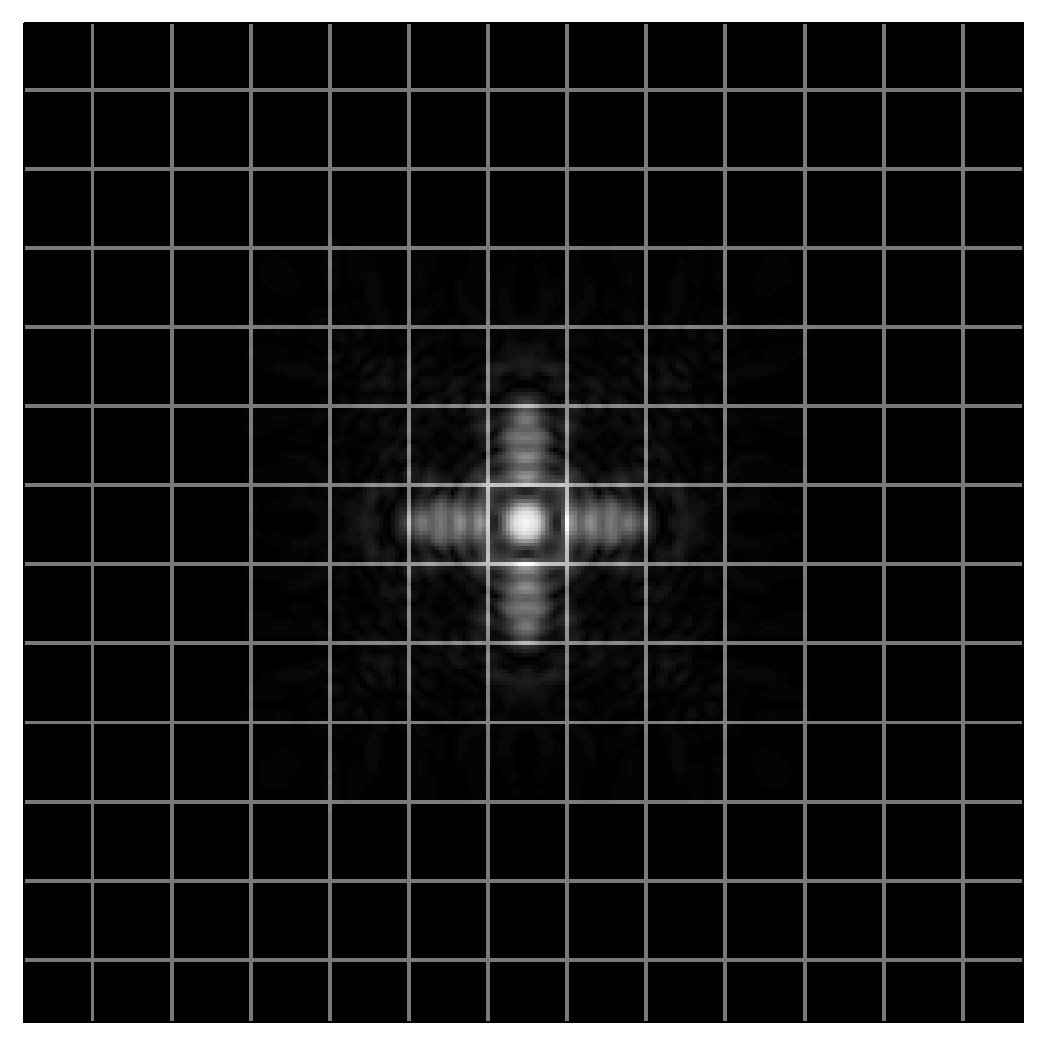
\includegraphics[width=.4\textwidth]{C:/Users/Massimo/Documents/Thesis/Thesis_PhD/crosstalk1.eps}
	\caption{\label{fig:crosstalk1} Raw plenoptic image of a point source. The grid represents the edges of the sub images. If the point source is in focus, it should be represented by only one lenslet. Because of diffraction some light goes also on the neighbouring sub images. }
\end{figure}
\begin{figure}[H]
	\centering
	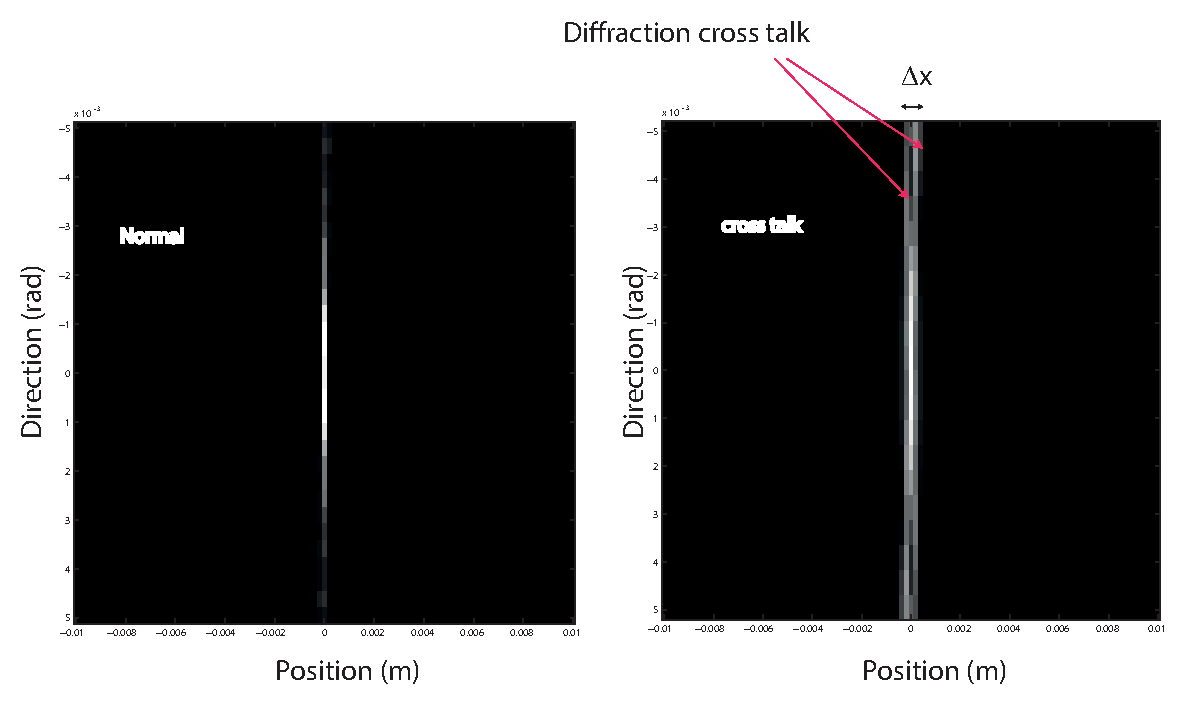
\includegraphics[width=1\textwidth]{C:/Users/Massimo/Documents/Thesis/Thesis_PhD/phasespacefocused2.eps}
	\caption{\label{fig:crosstalk2}Phase space of the light field of a point object: on the left is the case when the condition \ref{eq:min_diam} is respected; on the right when diffraction induces cross talk that arises between neighbouring lenslets. Cross talk introduces a blur in the rendered image whose width is $\Delta x$. }
\end{figure}
Figure \ref{fig:crosstalk2} shows what happens in the phase space of a point source in the presence of cross talk and without cross talk. In the first case there is no blur since all the light coming from a point source in focus is recorded by a single lenslet, while in the second case the spreading of the light due to diffraction causes a blur that is proportional to the number of sub images involved. 
\section{Advanced Rendering Techniques}
As described in chapter \ref{chap:chapter1}, one pixel in the rendered image is obtained from the mean of all the pixels of the sub image that corresponds to the position of the pixel in the final image \cite{ng2006digital}. This method generates an image that is equivalent to the image obtained with a conventional camera without any additional information. Since the final resolution depends on the number of lenslets in the micro array, it will be smaller than the resolution that can be obtained by a conventional camera which instead uses the full sensor resolution \cite{georgiev2010focused}. To use the full variety of features enabled by light field imaging, more advanced post processing techniques of the raw data should be used. The first two post processing features presented are the change of aperture and of point of view. These effects are achieved by integrating each sub image along a sub set of directional coordinates, hence on a smaller number of pixels. 
\subsection{Changing Aperture}
The quality of the image captured by a conventional camera depends on the combination of shutter speed and aperture chosen in order to get the optimum total exposure \cite{pedrotti1993introduction}.
 The possibility of changing the aperture of the main lens in post processing allows us to change the depth of field of the final image. In the simulations presented in this work the shutter speed is not an issue since all the objects imaged static with constant and uniform illumination. Therefore what determines the exposure is the aperture of the main lens or the f-number. The f-number is proportional to the depth of field of the imaging system that can be defined as the range of depths that appears sharp in the resulting photograph \cite{ng2006digital}. If the f-number increases and the aperture gets smaller, the depth of field increases. Therefore a plenoptic camera can control the depth of field in post processing.
 Looking at the raw plenoptic image, each sub image is formed by a number of samples of the directions of the rays. If in equation \ref{eq:rendering2} the range of integration along the directional coordinates is reduced, the aperture of the main lens is reduced at the same amount. If the aperture is smaller the rays propagating with a large angle with respect to the optical axis will not reach the sensor and will be not considered to form the intensity of each pixel. The result is a rendered image that looks like it has been captured with a narrower aperture. Computationally the algorithm to reduce the aperture is:
 \begin{equation}
 	\label{eq:rendering4}
 	I(x,y) = \dfrac{1}{N'^2}\sum_{i=k_x/2}^{N-\frac{k_x}{2}}\sum_{j=k_{y}/2}^{N-\frac{k_y}{2}} L(x,y,i,j)
 \end{equation}
 where $N'=N-k$ and \textit{k} is the range of directional coordinates considered in the sum. This operation in the phase space is shown in figure \ref{fig:rendering4}:
 \begin{figure}[H]
 	\centering
 	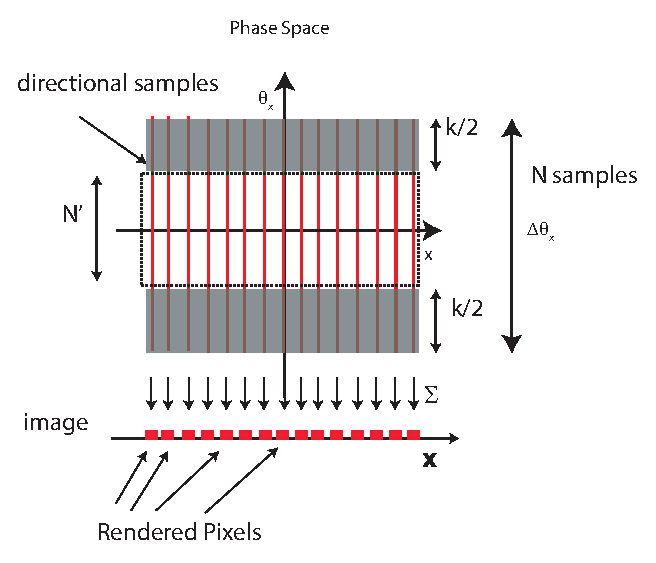
\includegraphics[width=.7\textwidth]{C:/Users/Massimo/Documents/Thesis/Thesis_PhD/renderingape.eps}
 	\caption{\label{fig:rendering4} Rendering seen from the $(x,\theta_x)$ slice of the phase space. The directional pixels not considered for the integration are shown in grey. }
 \end{figure}
An effect of reducing the aperture of a camera is to extend its depth of field. Therefore the depth of field can be digitally extended changing the range of directional coordinates included in the sum as explained above.
Figure \ref{fig:rawstanford1} shows the raw image of thin silky skin separating two layers of an onion, immersed in oil to improve transparency. The image is obtained from the online repository of raw plenoptic data provided by Levoy in Syanford University \cite{levoy2006microscope}. 
 Figure shows \ref{fig:stanford1} the differences between the rendered image integrating over the full aperture, and the rendered image obtained using only the central pixel of each sub image. The effect is to reduce the aperture to a pinhole and to have an all-in-focus image.
 Images has been obtained with home made rendering algorithm written in MATLAB.
 \begin{figure}[H]
 	\centering
 	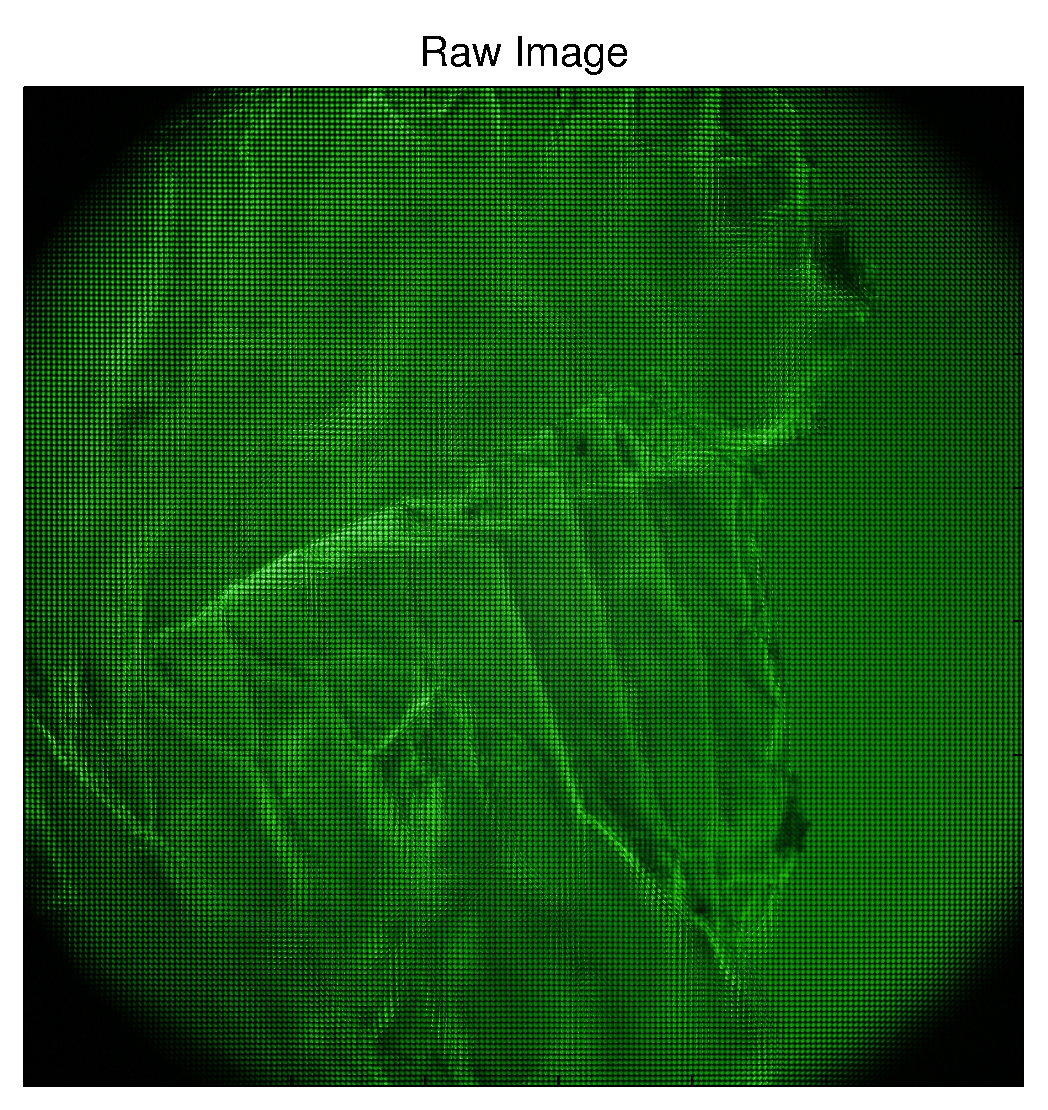
\includegraphics[width=.4\textwidth]{C:/Users/Massimo/Documents/Thesis/Thesis_PhD/rawst.eps}
 	\caption{\label{fig:rawstanford1} Raw plenoptic 1.0 image obatined from Levoy \textit{et al.} The microscope was a Zeiss Axiovert with a 20x/0.5NA (dry) objective. The micro lens array was 24mm x 36mm, with square 125-micron x 125-micron f/20 micro lenses, held in front of the Axiovert's side camera port using an optical bench mount. The camera was a Canon 5D full-frame digital SLR. The specimen was the thin silky skin separating two layers of an onion, immersed in oil to improve transparency \cite{levoy2006microscope}. }
 \end{figure}
\begin{figure}[H]
	\centering
	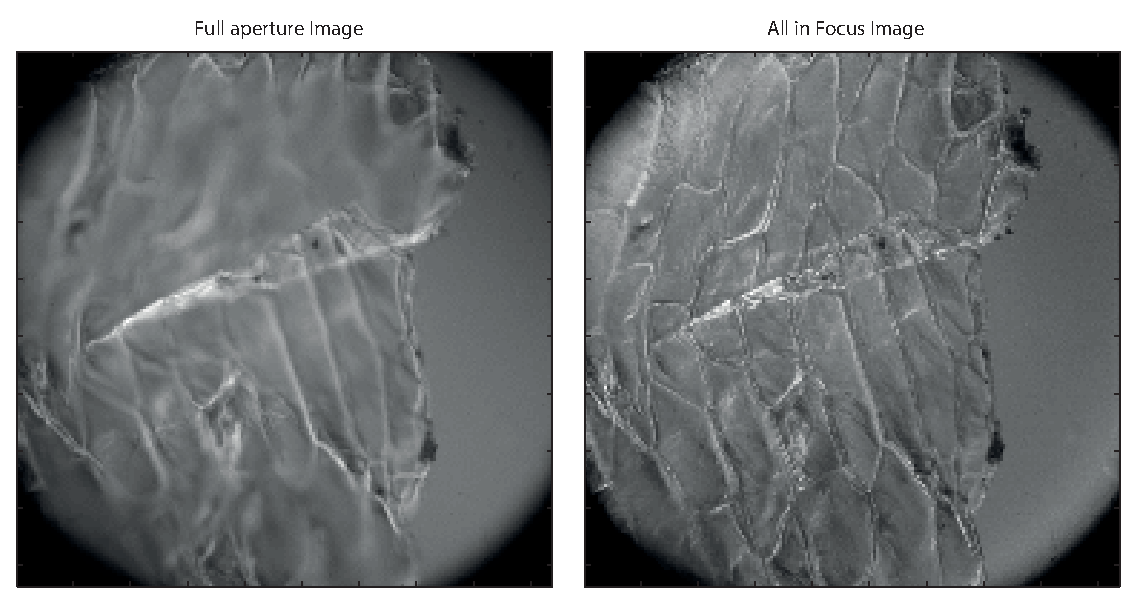
\includegraphics[width=0.9\textwidth]{C:/Users/Massimo/Documents/Thesis/Thesis_PhD/stanfordfull.eps}
	\caption{\label{fig:stanford1}Rendered Images from the raw data in figure \ref{fig:rawstanford1}. On the left there is the full aperture image obtained integrating along all the directional coordinates, while on the right there is the all in focus image obtained taking only the central pixel of the each sub image, that corresponds to rays with the direction parallel to the optical axis.}
\end{figure}
Reducing the number of pixel used to form the final image reduces of course the SNR of the image making it more noisy.
 \subsection{Changing the Point of View}
It is possible to change the point of view in the rendered image integrating along all the directional coordinates in one direction keeping fixed the other direction. For example an image corresponding to a particular point of view can be obtained, with reference to equations \ref{eq:rendering5}, keeping fixed the directional coordinate corresponding to the desired point of view and integrating along all the other coordinates. 
 \begin{equation}
 \label{eq:rendering5}
 \begin{matrix}
 I(x,y)=\dfrac{1}{N}\sum_{i=0}^{N} L(x,y,i,k_y) \\
 \\
 I(x,y)=\dfrac{1}{N}\sum_{j=0}^{N} L(x,y,k_x,j)
 \end{matrix} 
 \end{equation}
 \section{Depth Estimation}
 \label{sec:depth10}
 This section discuss how depth information can be extracted from light field data. In the specific case of plenoptic 1.0 raw data, depth can be decoded looking at the phase space. Section \ref{sec:phase_space} explained that a point source on the focal plane of the main lens looks like a straight vertical line in the phase space. The physical meaning of this is that for a single position, that is one lenslet, all the directional coordinates are sampled \cite{georgiev2010focused}. If the point source is out of focus the situation is different. If the source is closer to the main lens with respect to the focal plane, it will be imaged on a plane that is behind the micro array. This situation is shown in figure \ref{fig:depth}. Both directional and positional coordinates are sampled by more than one lenslet and each sub image will sample a set of directional coordinates corresponding to the part of the main lens from where the rays come. Figure \ref{fig:depth1} shows what happens in the phase space. On the lenslet plane the spot size will have a width of $\Delta x$ proportional to the distance, therefore the directions will be sampled by the lenslets included in this interval. Each lenslet receives light coming  a particular area of the main lens, its correspondent sub image only records the pixels linked with those coordinates as can be seen comparing figure \ref{fig:depth} with \ref{fig:depth1}. The resultant phase space representation is still a straight line, but with positive slope proportional to the distance of the point source \ref{fig:depth1}. If the source is further away from the plane where the main lens is focused, the main lens image is formed before the lenslets plane. The point is still sampled by more than one lenslet included in the spot size $\Delta x$. The difference with the previous case is that now in the phase space the point source is represented by a straight line with a negative slope. The physical meaning of the slope of the phase space line can be understood by looking at figure \ref{fig:depth3}. When the main lens image is formed in front of the micro lens plane the increasing values of $\theta_x$ axis are mapped on decreasing values of x and the line on the phase space representing the point has a negative slope. If the image is formed behind the micro lens plane increasing directions on $\theta_x$ axis are mapped on increasing positions on the x axis this inversion is absent and the line in the phase space has a positive slope \cite{ng2006digital}. This characteristic of the phase space permits us to discriminate between points in the scene that are in front or behind the main lens focal plane, giving a first rough depth estimate. 
 \begin{figure}[H]
 	\centering
 	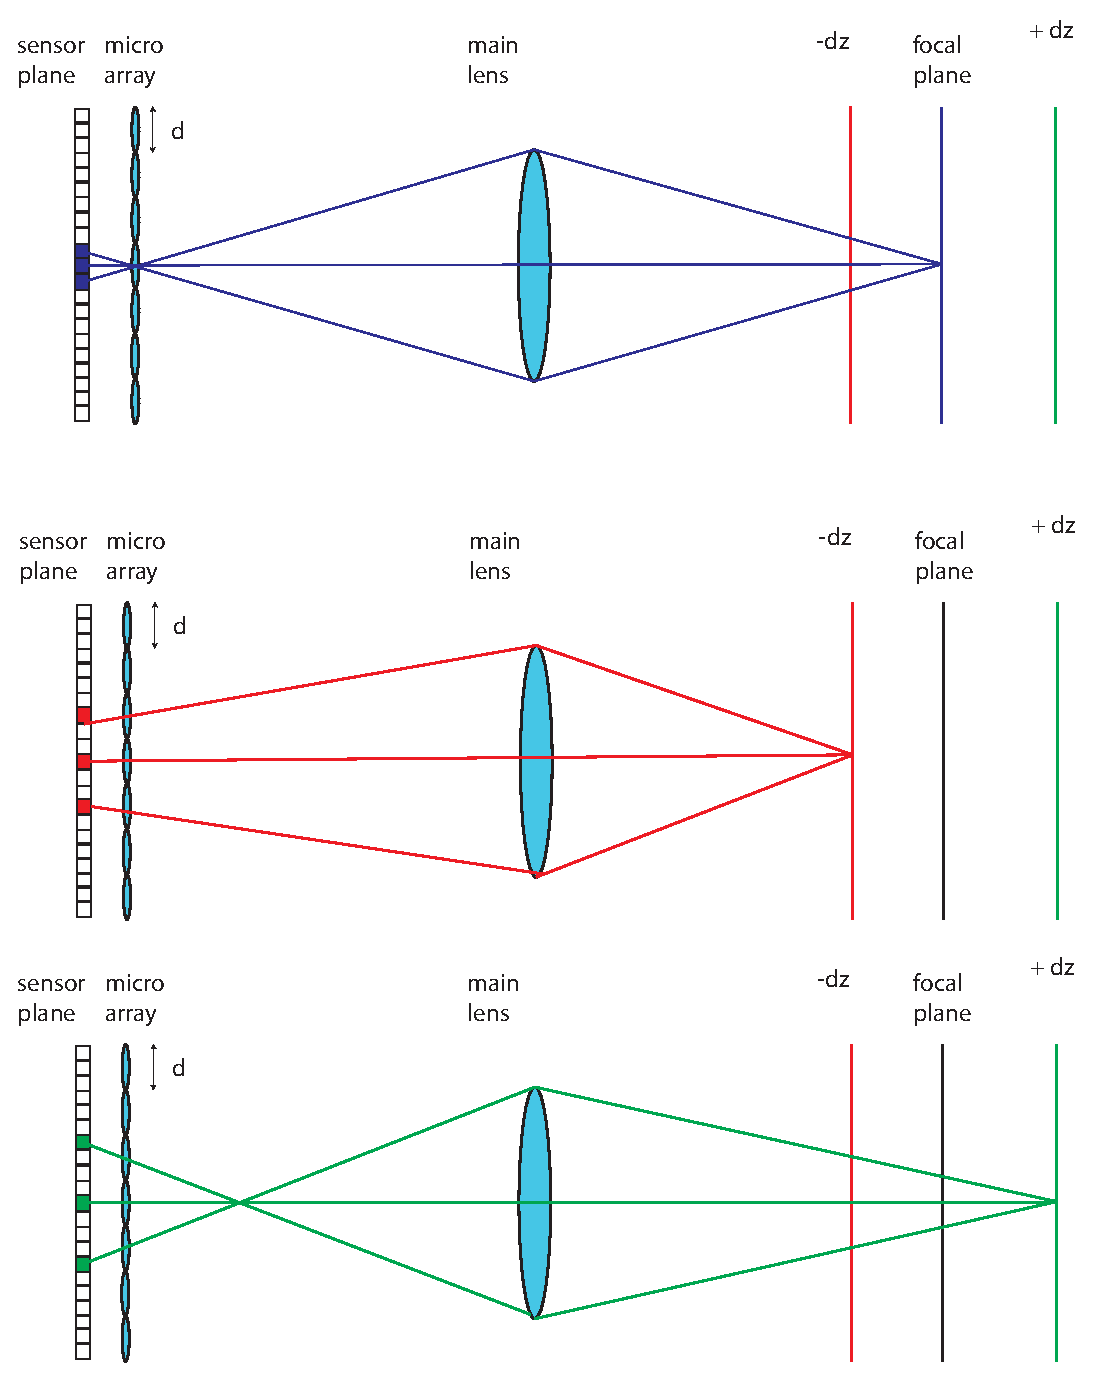
\includegraphics[width=.9\textwidth]{C:/Users/Massimo/Documents/Thesis/Thesis_PhD/defocous10.eps}
 	\caption{\label{fig:depth} Sampling of the light field of a point source in focus, on the top, closer to the main lens, centre, and further away, bottom. When the source is out of focus, both position and directions are sampled by more than one lenslet since the main lens image is no longer formed any more on the lenslet plane. }
 \end{figure}
 \begin{figure}[H]
 	\centering
 	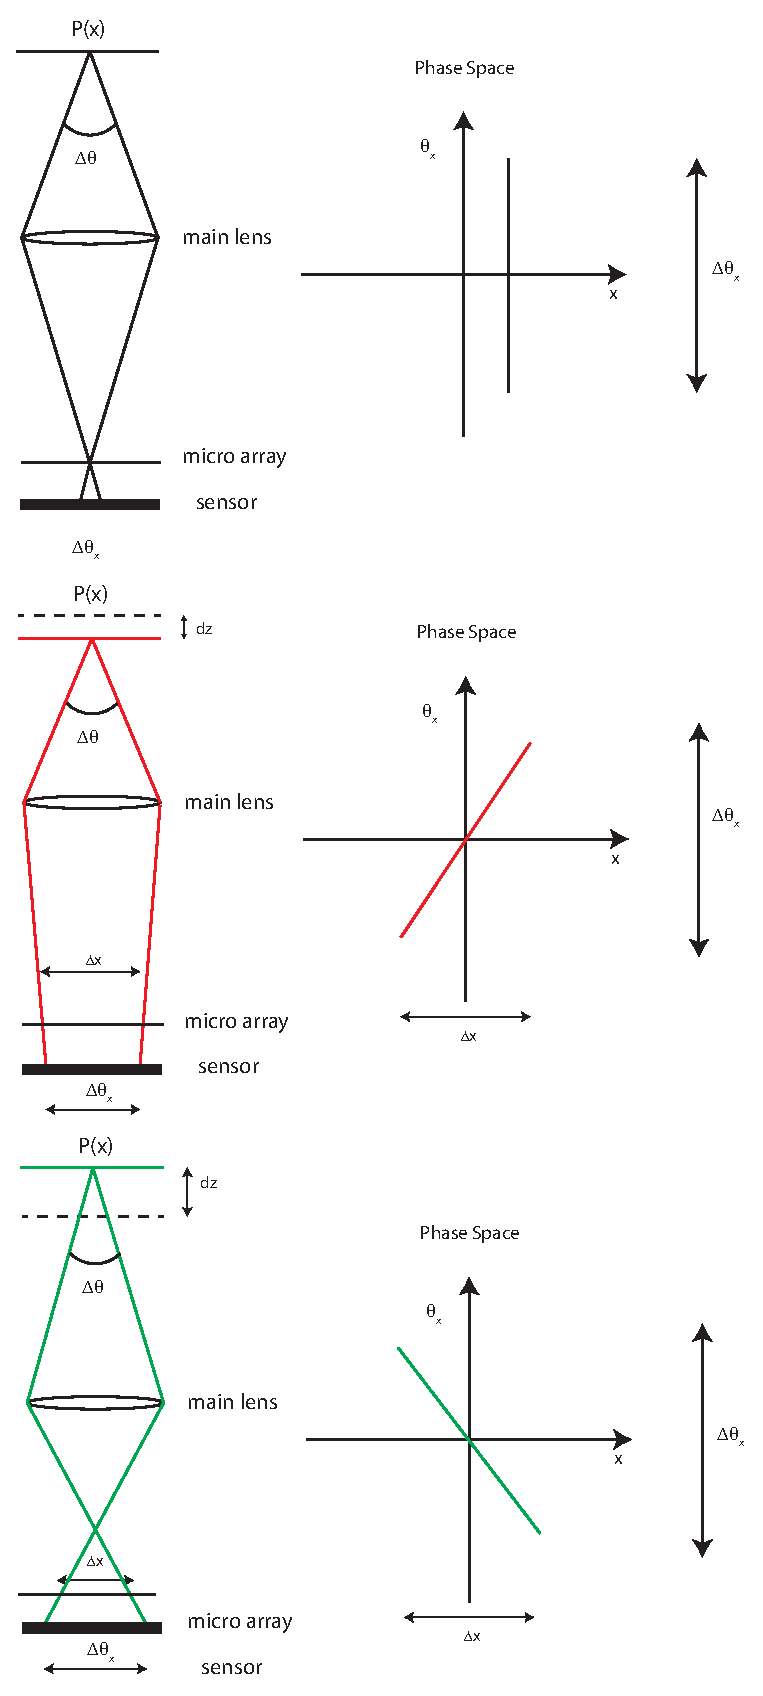
\includegraphics[width=.6\textwidth]{C:/Users/Massimo/Documents/Thesis/Thesis_PhD/phasespacerefocus10.eps}
 	\caption{\label{fig:depth1} Information on the depth of a point source imaged by a plenoptic 1.0 system. As explained in section \ref{sec:phase_space}. If the point source is in focus, on the top, its position is sampled by one lenslet as well as the whole set of directions.}
 \end{figure}
 \begin{figure}[H]
 	\centering
 	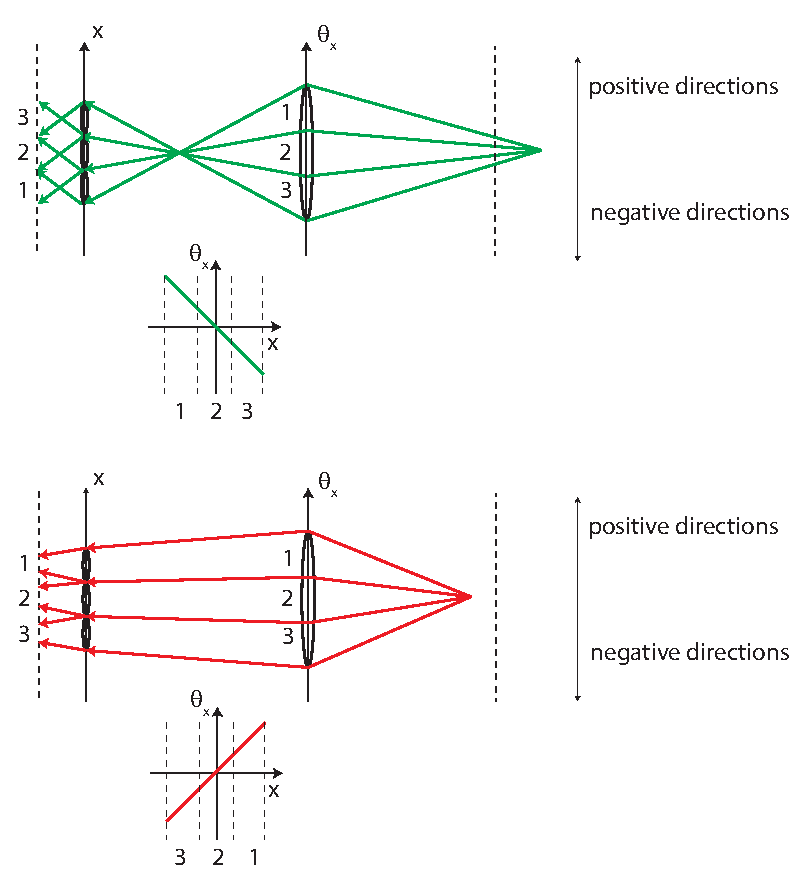
\includegraphics[width=.7\textwidth]{C:/Users/Massimo/Documents/Thesis/Thesis_PhD/slope.eps}
 	\caption{\label{fig:depth3} Physical meaning of the slope in the phase space. If the point source is further then the camera focal plane, the phase space line has a negative slope. If the point source is closer then the focal plane, the slope of the phase space line is positive.}
 \end{figure}
 Plenoptic 1.0 camera simulations, as discussed above, have been run to verify this fact. The system was composed of a main lens with a focal length of \textit{120 mm}, in a \textit{2f} configuration creating an image on the micro array plane. The Micro lens array was composed of a matrix of 101 $\times$ 101 lenslets with a diameter of 100 $\mu m$ and a focal length of 100 \textit{mm}. The ensor had a resolution of 200 by 2000 pixels.
 \begin{figure}[H]
 	\centering
 	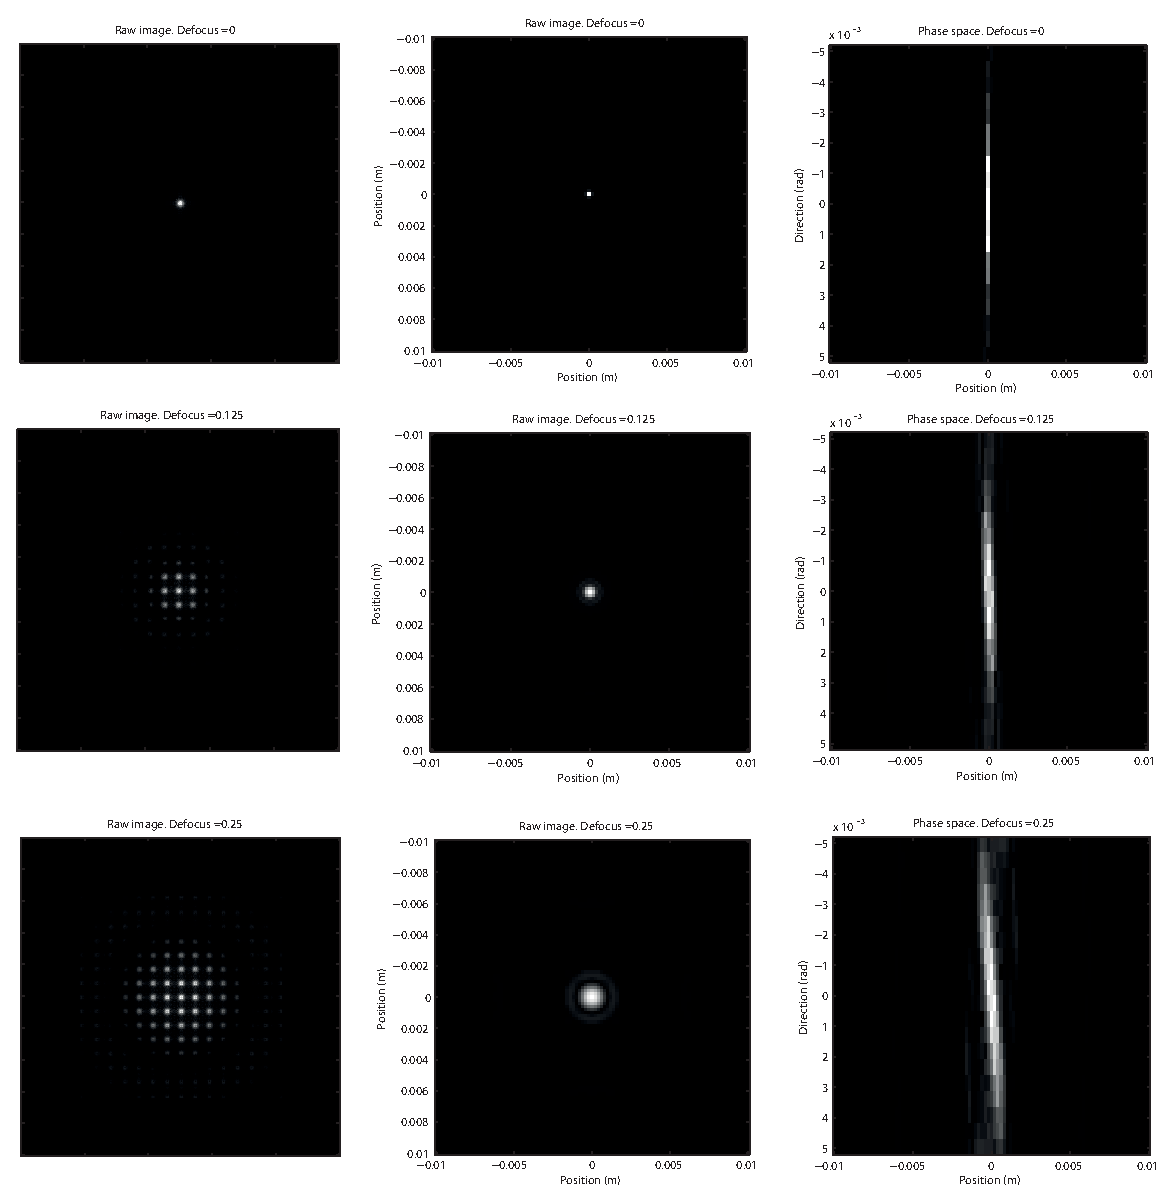
\includegraphics[width=.7\textwidth]{C:/Users/Massimo/Documents/Thesis/Thesis_PhD/defocus10.eps}
 	\caption{\label{fig:depth4} Numerical simulation of a point source imaged by a plenoptic 1.0 imaging system. The point source was placed at three different distances from the main lens. The top three figures show the focused image. In the centre ones a defocus of 0.125 m closer to the main lens is added. In the bottom ones the point source is closer to the main lens of 0.25 m. In all the three cases the raw data image is on the left, the rendered image is on the centre and the phase space line is on the right.}
 \end{figure}
 \newpage
 \section{Synthetic Refocus}
 \label{sec:refocus10}
Another post processing feature enabled by collecting the light field is the possibility to refocus an image after it has been captured. This features is called synthetic refocusing and is based on the fact that the recorded light field can be used to compute images as if they were taken by a synthetic camera positioned and focused differently from the actual camera. In this section the synthetic refocusing algorithm is explained in terms of the discussion in Ng \cite{ng2006digital} and Ng \textit{et al.} \cite{ng2005light}. \\
This method is based on the fact that for a plane out of focus for the real camera, it is possible to define a synthetic camera composed of an aperture and a sensor plane that is focused on that particular plane. The image produced by the synthetic camera will result in focus. This method is based on a synthetic camera model obtained with ray tracing. It can be implemented in a wave optics approach using the simulation platform developed in this work and the limitations and the issues arising from a wave approach with respect to the simple and ideal ray optics approach will be discussed. 
 Figure  \ref{fig:synthetic0} shows a plenoptic 1.0 imaging system whose main lens produces an out of focus image on the micro lens plane. The directional set of coordinates $\Delta u$ is mapped along the range of spatial coordinates $\Delta x$. The light field can be reparametrized in terms of a synthetic light field generated by an aperture on the plane \textit{u'} represented by the dashed lens, that focuses the object on a synthetic focal plane, \textit{x'}. This second light field is parametrized with the coordinates \textit{u' v'} and \textit{x' y'}. 
 \newpage
 \begin{figure}[H]
 	\centering
 	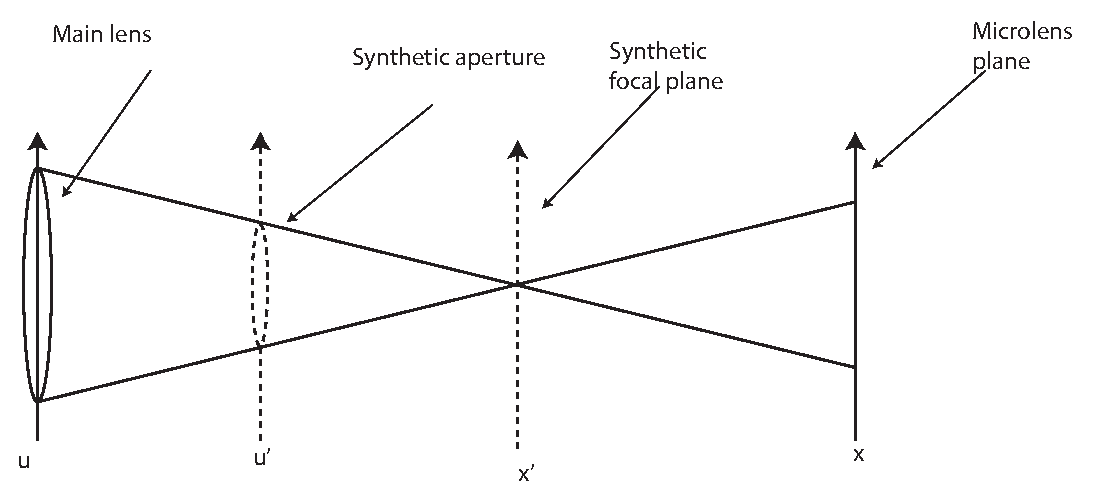
\includegraphics[width=.8\textwidth]{C:/Users/Massimo/Documents/Thesis/Thesis_PhD/sinth0.eps}
 	\caption{\label{fig:synthetic0} The synthetic camera refocusing method is based on the fact that is always possible to define a virtual aperture that is focused on the lenslet plane. }
 \end{figure}
 As explained by Ng \textit{et al.} \cite{ng2005light} and in analogy with what was explained in section \ref{sec:rendering1} it is possible to define the intensity obtained rendering a synthetic light field $L'(x',y', u', v') $ at the synthetic focal plane as:
 \begin{equation}
 \label{eq:sinth1}
 I(x,y)=\iint L'(x',y',u',v')A(u',v') du'dv'
 \end{equation}
 The goal is to express this intensity as a function of the captured light field $L(x,y,u,v)$ present on the actual sensor plane, finding the relationship that links the set of coordinates \textit{x, y, u, v} with \textit{x', y', u', v'}. 
 \newpage
 \subsection{Synthetic Refocus Algorithm}
 This algorithm has been developed by Ng \textit{et al.} \cite{ng2005light}. To find the link between the real and the synthetic light field the following simplifications are made: 
 \begin{itemize}
 	\item only the synthetic sensor plane \textit{x', y'} will be moved. Therefore the main lens plane \textit{u', v'} is at the same position of the plane \textit{u, v}, and no transformation is performed on the directional coordinates, therefore (\textit{u, v})=(\textit{u', v'}).
 	\item the aperture of the main lens will not change, $A(x', y')=1$.
 \end{itemize} 
 Figure \ref{fig:synthetic3} shows a two dimensional diagram explaining the reparametrization under the simplifications explained above. Only the coordinates x and u are shown for simplicity. F is defined as the distance of the main lens from the lenslet array plane, and F' as the distance from the synthetic focal plane. The ratio between these two distances is the refocusing parameter $ \alpha'$, defined as: 
 \begin{equation}
 	\label{eq:alpha}
 	 \alpha' = \dfrac{F}{F'}
 \end{equation}
 The refocusing factor can assume the following values:
 \begin{itemize}
 	\item $ \alpha'=1$ when the synthetic focal plane is at the same position of the main lens focal plane
 	\item $ \alpha'>1$ when the distance between the main lens and the synthetic 
 	image plane is smaller than the distance between the main lens and its original focal plane. This occurs when the system is refocused on a plane that it is further away with respect to the main lens focal plane.
 	\item $ \alpha'<1$ when the distance between the main lens and the synthetic image plane is bigger than the distance between the main lens and its original focal plane. This occurs when the refocus takes place on a plane that is closer with respect to the main lens.
 \end{itemize}
 \begin{figure}[H]
 	\centering
 	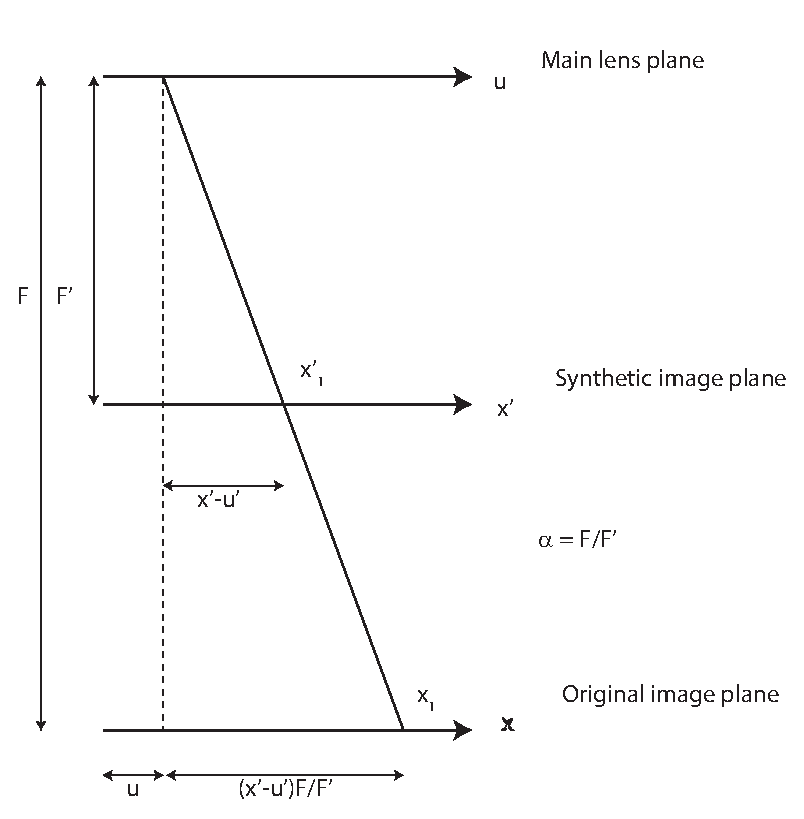
\includegraphics[width=.8\textwidth]{C:/Users/Massimo/Documents/Thesis/Thesis_PhD/refocus2.eps}
 	\caption{\label{fig:synthetic3} Changing the focal plane of the camera is equal to re-parametrizing the light field according to the new coordinates. The re-parametrization corresponds to a scaling of the ratio between the refocused plane and the original camera plane $ \alpha'$. }
 \end{figure}
 Looking at figure \ref{fig:synthetic3} a ray of light that crosses the main lens plane at the coordinate $u$ and that then intercepts the synthetic image plane at the point $x'_1$, can be represented with the coordinates of the original image plane $x_1$. Because of similar triangles, the value of the \textit{x} coordinate on the image plane can be expressed as a function of the coordinates $ u, x'$:
 \begin{equation}
 	\label{eq:refocus11}
 	x_1 = u+(x'_1-u)\dfrac{F}{F'}=u+(x'_1-u) \alpha'
 \end{equation}
 Therefore extending to the four dimensional case, the points belonging to the synthetic image plane can be expressed as a function of the directional coordinates at the main lens plane and the spatial coordinates at the original image plane as:
 \begin{equation}
 \label{eq:shear1}
 \begin{matrix}
 x' = \dfrac{x}{ \alpha'}+u\left(1-\dfrac{1}{ \alpha'}\right) \\
 \\
 y' = \dfrac{y}{ \alpha'}+v\left(1-\dfrac{1}{ \alpha'}\right)
 \end{matrix} 
 \end{equation}
 With this change of coordinates the light field at the synthetic focal plane $x'$ can be written substituting equations \ref{eq:shear1} into equation \ref{eq:sinth1}.
 \begin{equation}
 \label{eq:synthLF2}
 I(x,y) =\iint L\left(\dfrac{x}{ \alpha'}+u\left(1-\dfrac{1}{ \alpha'}\right),\dfrac{y}{ \alpha'}+v\left(1-\dfrac{1}{ \alpha'}\right),u,v\right)A(x',y')dudv
 \end{equation}
 Equation \ref{eq:synthLF2} represents the rendered image obtained by integrating along the directional coordinates of the light field reparametrized as if it were captured by a camera whose focal plane is the same as the synthetic focal plane. \\
 Focusing at different depths corresponds to changing the separation between the lens and the image plane, shifting it by a quantity proportional to the refocusing factor $ \alpha'$. From equation \ref{eq:shear1} the four dimensional light field at the synthetic plane is obtained from the light field recorded on the sensor by shifting and rescaling its spatial coordinates. The transformation operated on the light field is the composition of two transformations:
 \begin{itemize}
 	\item a scaling of a factor $ \alpha'$ that depends on the distance of the synthetic focal plane from the main lens.
 	\item a translation term $u(1-1/ \alpha')$ that increases with the directional coordinates and with the magnitude of the factor $ \alpha'$.
 	 \end{itemize} 
 	 Therefore the synthetic refocus can be treated as a linear operator acting on the four dimensional light field that maps the light field recorded on a new set of coordinates. The rendering on this new set of coordinates gives the image focused at a different plane.
\subsection{Refocusing Operator}
The synthetic refocus equation \ref{eq:synthLF2} has been obtained with ray optics considerations only. However, it can be applied to light fields obtained with wave optics simulations. When using wave optics particular attention should be given in the design of the imaging system in order to avoid cross talk effects induced by diffraction, as explained in section \ref{sec:diffraction}. The effects of this operator in the phase space is a change of the slope of the lines describing the points of the image in the phase space. Since the total light field is conserved, the area in the phase space remains the same, hence the projection of the light field on the phase space is sheared with respect to the original one \cite{georgiev2010focused}.
\begin{figure}[H]
	\centering
	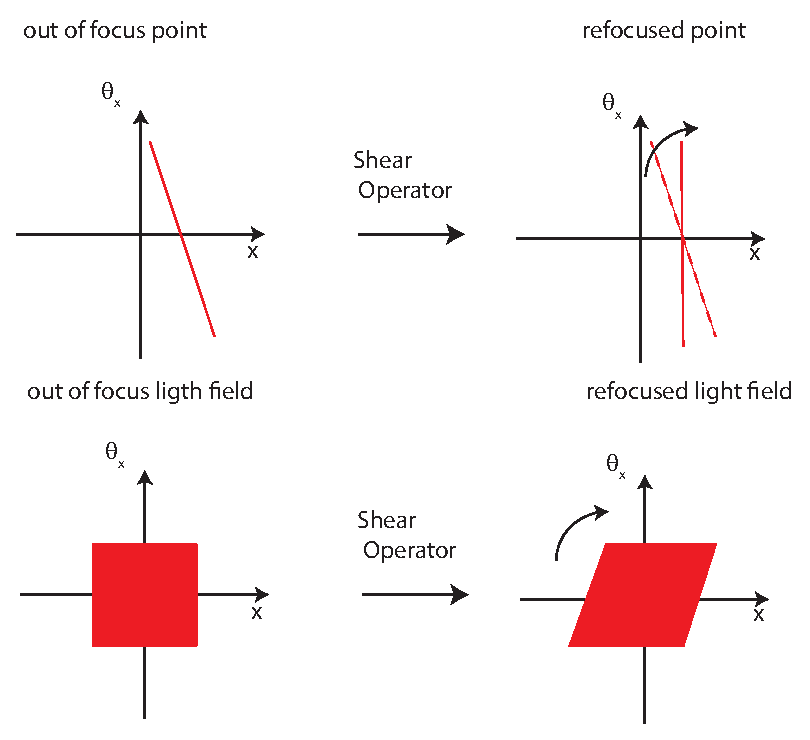
\includegraphics[width=.8\textwidth]{C:/Users/Massimo/Documents/Thesis/Thesis_PhD/shear1.eps}
	\caption{\label{fig:shear1} Changing the position of the focal plane is equal to shear the light field in the phase space. The total area remains the same since the total light field is conserved. }
\end{figure}
 MATLAB code has been developed to implement the synthetic refocus operator. The algorithm is composed of two distinct stages. The first stage creates a new set of spatial coordinates shifting and rescaling the original set of coordinates as shown in equation \ref{eq:shear1}. Then the output synthetic light field is created interpolating the input light field using as a base the new set of coordinates. The flow chart can be seen in figure \ref{fig:flowcharet1}

\begin{figure}[H]
	\centering
	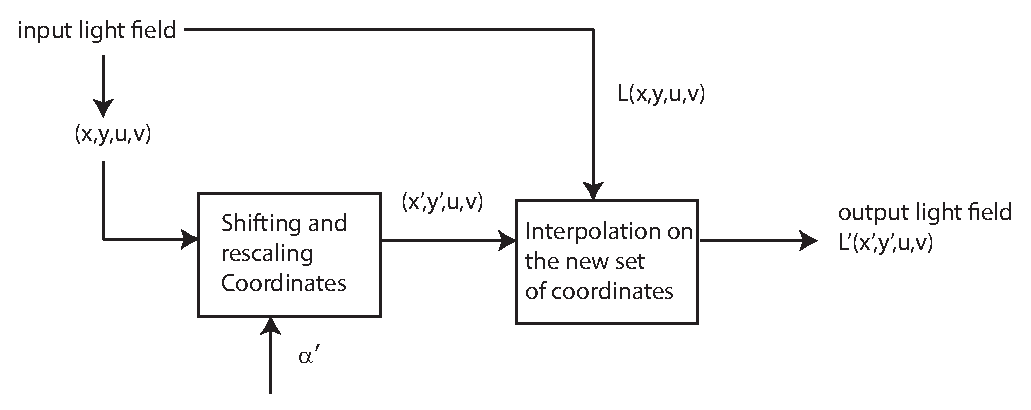
\includegraphics[width=.8\textwidth]{C:/Users/Massimo/Documents/Thesis/Thesis_PhD/flowshear.eps}
	\caption{\label{fig:flowcharet1} Flow chart of the operator shearing. }
\end{figure} 
\section{Results of the Simulations}
To test and explore the potentials of the synthetic refocusing algorithm the wave optics simulation toolbox described in section \ref{chap:fresnel} has been used. The System simulated is the one described in section \ref{sec:system} and shown in figure \ref{fig:pleno10_system2}. The optical parameters can be found in the following table. These parameters have been chosen in order to minimize the phase aliasing in the lens, to avoid diffraction induced cross-talk between the lenslets and to match the f-number of the main lens with the lenslets.
\\
\\
\begin{table}
	\centering
\begin{tabular}{l|r}

	Main lens focal length f & 120 mm\\ \hline
	Lens aperture D & 3.6 mm \\ \hline
	Micro lens focal length $f_{\mu}$ & 10 mm \\ \hline
	Micro lens diameter d & 150 $\mu m$ \\ \hline
	Micro array pitch p & 150 $\mu m$ \\ \hline
	Sensor size & 20 mm \\ \hline
	f-number & 33.6\\ \hline
	sensor resolution & 3030 by 3030 pixel \\ \hline	
%   
\end{tabular}
\caption{\label{tab:1} Simulations parameters. }
\end{table}

\begin{figure}[H]
	\centering
	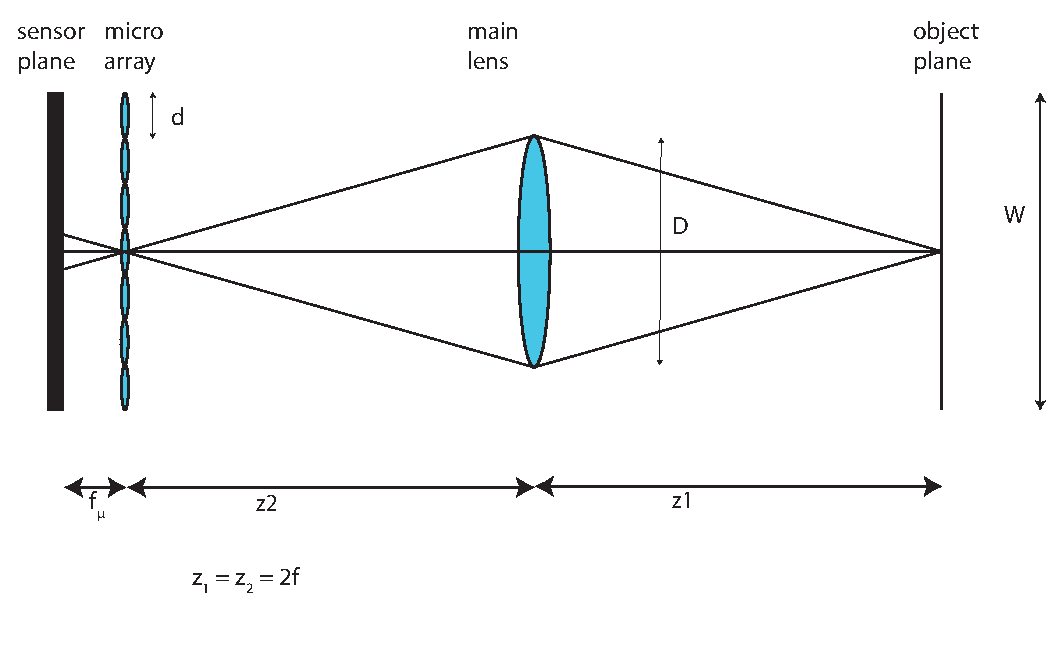
\includegraphics[width=.7\textwidth]{C:/Users/Massimo/Documents/Thesis/Thesis_PhD/plenoptic101.eps}
	\caption{\label{fig:pleno10_system2} Set up of a plenoptic 1.0 camera replicated in the simulations. }
\end{figure}		
With this set up the final rendered image resolution iss 101 $\times$ 101 pixel. Each pixel of the final image corresponds to a lenslet, therefore the spatial resolution the final image is equal to the diameter of a single lenslet. Each sub image has 30 $\times$ 30 pixels, meaning that the full set of directional coordinates is sampled by $N_{sub}=30$ samples. The angular resolution is therefore:
\begin{equation}
\label{eq:angularres}
\delta\theta = \dfrac{\Delta\theta}{N_{sub}}=\dfrac{NA}{N_{sub}}
\end{equation}
and is equal to $\delta\theta = 2.5 10^{-4} rad$.\\
The first object to be imaged was a volume V of dimension 20 mm $\times$ 20 mm $\times$ 100 mm containing three point sources. Each point source has been simulated by a circle of 10 $\mu m$ diameter and are positioned as shown in figure \ref{fig:volumepoint}
\begin{figure}[H]
	\centering
	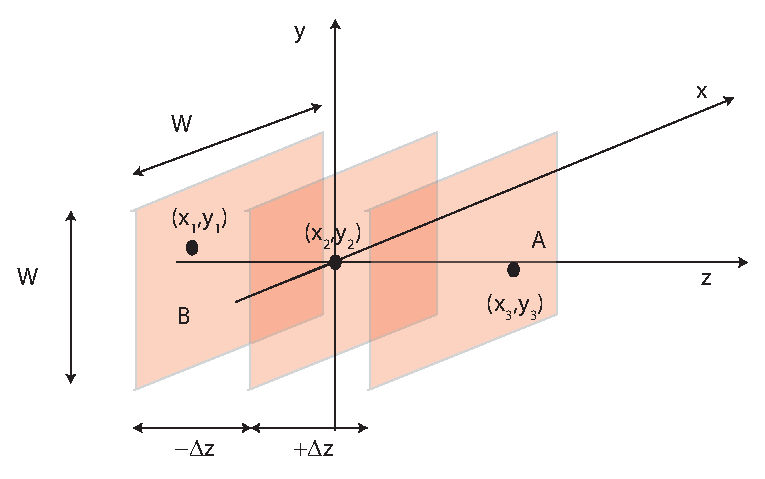
\includegraphics[width=.7\textwidth]{C:/Users/Massimo/Documents/Thesis/Thesis_PhD/planes.eps}
	\caption{\label{fig:volumepoint} Position of the point sources imaged inside the volume V simulated. The planes B and A are the boundaries of the volume considered. }
\end{figure}
Each plane has been imaged independently setting the distance $z_1$ equal to the sum of the distance of the main lens focal plane and the defocus $\delta z$. The Coordinates of the points are: 
\begin{itemize}
	\item A: $x_1 = -3 mm , \quad y_1 = -3 mm , \quad z_1 = -50 mm$
	\item B: $x_2 = 0 mm, \quad y_2 = 0 mm, \quad z_2 = 0 mm$ 
	\item C: $x_3 = +3 mm , \quad y_3 = +3 mm, \quad z_3 = +50 mm$
	\end{itemize} 
Following the simulated propagation of the three planes through the system, the final output raw image has been obtained by summing the three separate raw images normalized by the total amount of energy contained. This can be done since the Fresnel simulation toolbox is time independent. Figure \ref{fig:rawandimage} shows the total raw image and the rendered image integrated without any refocusing.
\begin{figure}[H]
	\centering
	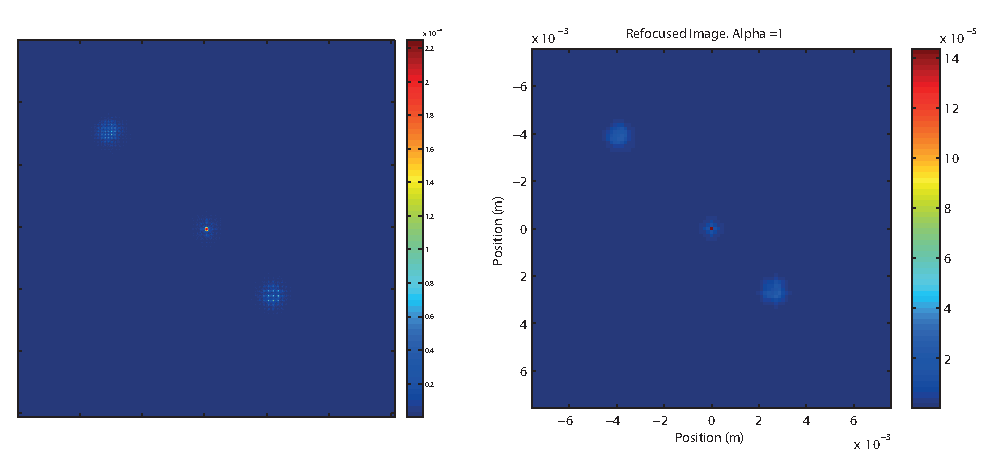
\includegraphics[width=.7\textwidth]{C:/Users/Massimo/Documents/Thesis/Thesis_PhD/refocus1.eps}
	\caption{\label{fig:rawandimage} Raw image on the left and rendered image on the right. Intensity is shown in false colour in order to appreciate variations in energy distribution. }
\end{figure}
The central spot is in focus, since the point source is at a distance of \textit{z = 2f} on the main lens focal plane.
For a defocus of 50 mm the factor $ \alpha'$ can be obtained from the lens equation. For the 2f system simulated and referring to figure \ref{fig:synthetic3} for notations:
\begin{equation}
\label{eq:alpha1}
\dfrac{1}{f} =\dfrac{1}{F'}+\dfrac{1}{(z+\Delta z)} 	
\end{equation}
Since $ \alpha' = F/F'$, and in a 2f system F=2f=z:
\begin{equation}
\label{eq:alpha2}
\dfrac{1}{f} =\dfrac{ \alpha'}{2f}+\dfrac{1}{(2f+\Delta z)} 	
\end{equation}
Resolving for $ \alpha'$ becomes:
\begin{equation}
\label{eq:alpha3}
 \alpha' = \dfrac{2f+s\Delta z}{2f+\Delta z} 	
\end{equation}
Figure \ref{fig:alpha} shows the values of $ \alpha'$ obtained by equation \ref{eq:alpha3} for defocus varying between plus and minus 10 cm.
\begin{figure}[H]
	\centering
	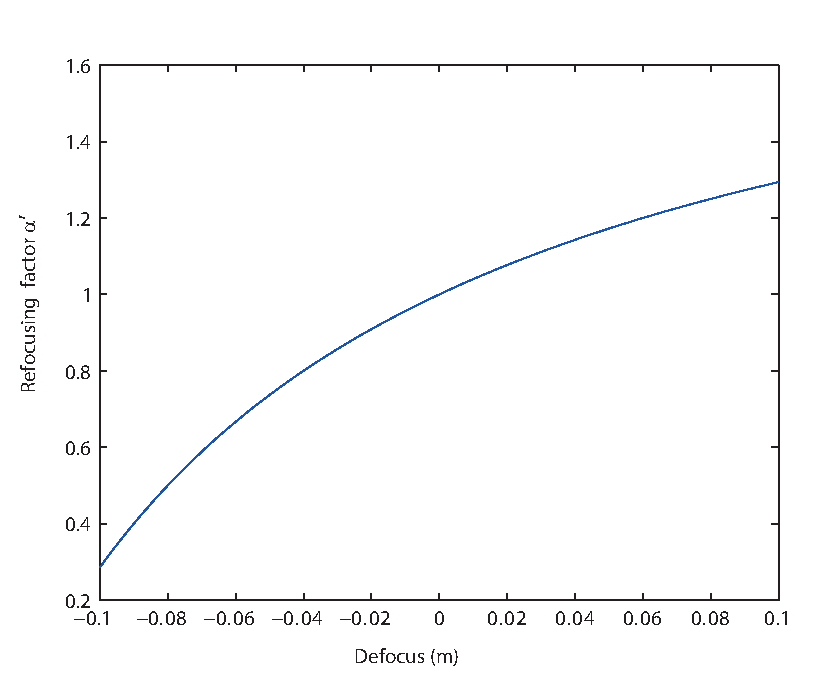
\includegraphics[width=.7\textwidth]{C:/Users/Massimo/Documents/Thesis/Thesis_PhD/alphadef.eps}
	\caption{\label{fig:alpha} Values of the refocusing factor $ \alpha'$ as a function of the defocus. A positive defocus means that the object it further away with respect to the main lens, a negative defocus indicates an object that is closer. }
\end{figure}
Figure \ref{fig:alpha} shows that, as expected, the refocus factor is not linear with defocus and therefore the axial resolution in not linear. When the object is closer to themain lens, small variations in the defocus give large variations in $ \alpha'$ while the opposite happens when the object is further away with respect to the main lens. \\
Figure \ref{fig:refocus} shows the refocused imaged obtained from shearing the light field extracted by the raw image in figure \ref{fig:rawandimage} on the left. According to equation \ref{eq:alpha3}, the point A is refocused for a value of $ \alpha'$ equal to 0.7 and point B for $ \alpha' = 1.17$.
\begin{figure}[H]
	\centering
	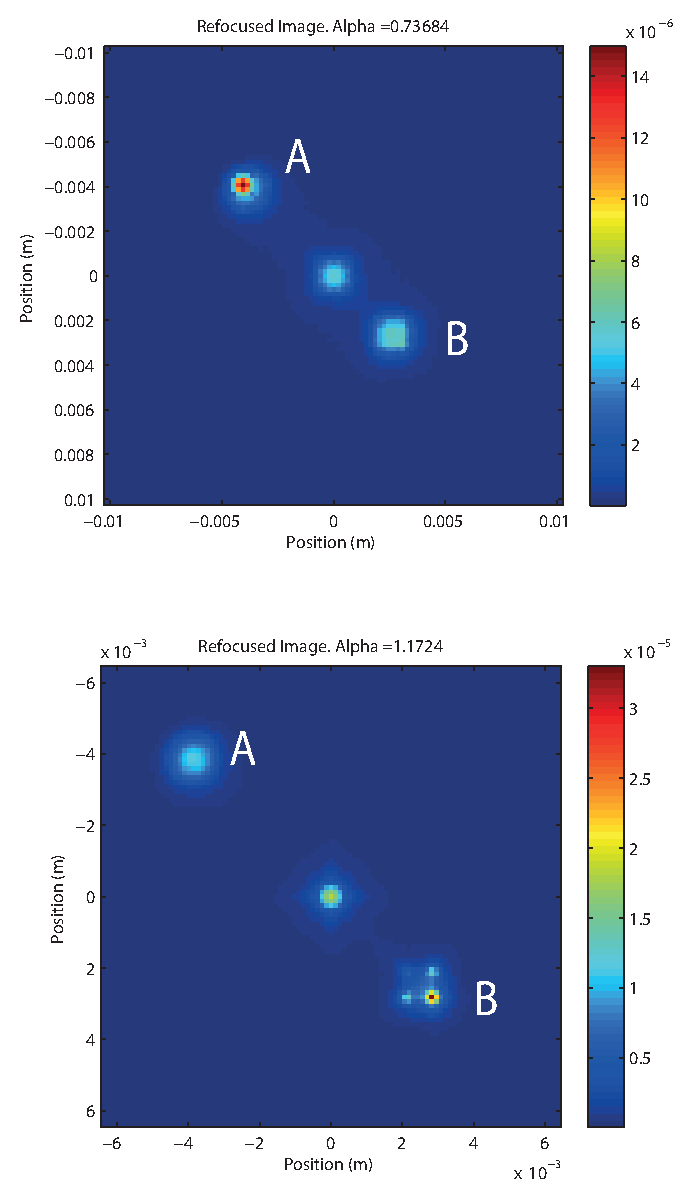
\includegraphics[width=.7\textwidth]{C:/Users/Massimo/Documents/Thesis/Thesis_PhD/refocus3point.eps}
	\caption{\label{fig:refocus} Refocused images of the three point sources in figure \ref{fig:rawandimage}. In the top one the point A is refocused, in the bottom one the point B is refocused. When the point source is refocused, the intensity distribution is higher with respect to the out of focus points. }
\end{figure}
The effects of the refocusing operator can be appreciated by looking the intensity values of the refocused point sources. In the top image of figure \ref{fig:refocus} the point labelled with the letter A is refocused, and the majority of the light present in the image concentrates on its location. The same happens in bottom figure, where the brightest point, indicated in red according to the colour bar, is the refocused one (B). This is a proof of the fact that the refocusing operator, shearing the four dimensional light field, moves the intensity from a location to another. The total energy of the image remains unchanged. 
\\
\section{Focal Stack Depth Estimation} 
The synthetic refocus algorithm provides a method to estimate the depth of a point source in a volume. This is an original contribution to the field and it is a proof of concept that depth information can be evaluated from the blur of the image. It has been treated only for the case of imaging a point source for simplicity. Further work should be done to extend it to larger more complex objects. Looking at the Fourier transform of a rendered image of a point source before and after the refocusing operation shows that when the point source is in focus, its spectrum is broader than the blurred one. This fact is true for general images as well, when the presence of sharp details in the focused image, causes its spectrum to have a larger amount of high spatial frequencies, and therefore more energy at high frequencies. Figure \ref{fig:spec1} is shows the difference between the spectrum of the out of focus image (blue) and the in focus image (red) for a defocus of 5 cm.
\begin{figure}[H]
	\centering
	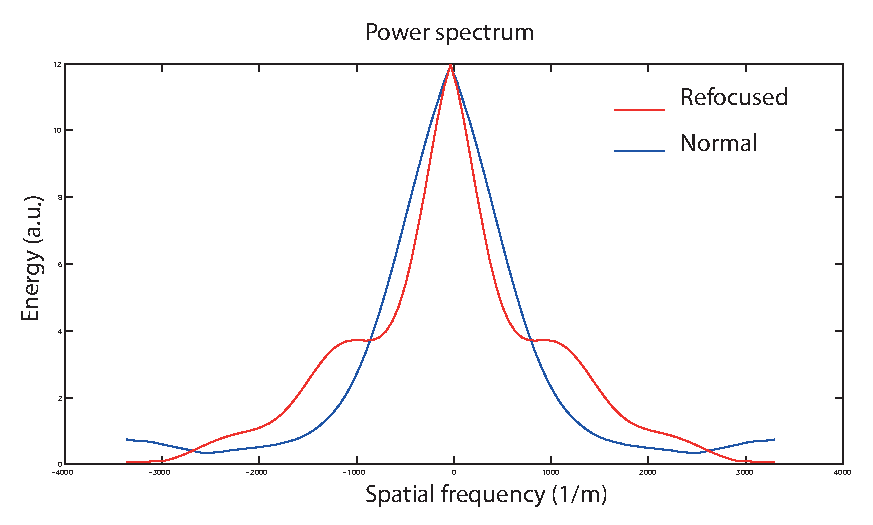
\includegraphics[width=1\textwidth]{C:/Users/Massimo/Documents/Thesis/Thesis_PhD/spectrum2.eps}
	\caption{\label{fig:spec1} Spectrum of out of focus image (blue) and spectrum of the refocused image (red). }
\end{figure}
The action of shearing the light field produces a redistribution of the power spectrum of the signal towards high frequencies. \\
 This effect can be used to estimate the depth of the object imaged by evaluating its level of blur. This blur based depth estimation is an original contribution of this work to light field literature. The method consists in creating a focal stack by shearing the light field at different values of the coefficient $ \alpha'$, that correspond to different focal planes, and rendering the images. After the focal stack is created the power spectrum of each image is calculated using the fast Fourier transform algorithm. The low frequency terms are then removed by high pass filtering the images and the total energy contained in the high frequency term is calculated by integrating the Fourier spectra. The bandwidth of the high pass filter has been calculated in order to remove the central lobe of the spectrum. Plotting the values of energy as a function of the different $ \alpha'$ coefficients a curve with a maximum in the proximity of the most in focus image is obtained. This maximum corresponds to the image in the focal stack that best estimates the actual value of $ \alpha'$. Figure \ref{fig:maxima} shows the energy as a function of the refocus parameter $ \alpha'$ for a point source placed at different depths. The vertical red line indicates the position of the maximum. The values of the estimated $ \alpha'$ and the real one are shown in table \ref{tab:alphaest}.

 \begin{table}
 	\label{tab:alphaest}
 	\begin{center}
  \begin{tabular}{l|c|c|r}
  	\hline
  	Estimated $ \alpha'$ & Real $ \alpha'$ & Error & Defocus \\ \hline
  	0.85 & 0.738 & 0.1132 & -0.05 m\\ \hline
  	0.925 & 0.8837 & 0.0413 & -0.025 m\\ \hline 
  	1.080 & 1.0943 & -0.0143 & +0.025 m\\ \hline
  	1.105 & 1.1724 & 0.0674 & +0.05 m\\ \hline
  	\label{tab:2}
  \end{tabular}
\end{center}
  \caption{Comparison between the estimated and the real values of the refocusing factor $ \alpha$ }
 \end{table}

Figure \ref{fig:error} shows the distribution of the estimated values of $ \alpha'$ versus the actual values obtained from equation \ref{eq:alpha3}.
 The estimated values for a defocus of -0.1 m and - 0.08 m are equal to 1 as if the image would lie on the focal plane. These are clearly wrong estimations and represent a limitation for the method described. It is interesting to see that for negative defocus the parameter $ \alpha'$ is over estimated and the error is positive while for positive defocus the error is negative. The minimum error is present for values of defocus corresponding to positions close to the focal plane. The error in the estimation of the refocusing factor is plotted in figure \ref{fig:error1}.
 \\
 Having seen these results the method has a better accuracy in a range of depth around the focal plane and performs worse when the absolute value of the defocus increases.
 These results show that the depth evaluation depends on the distance of the object from the camera. This is a natural consequence of the non linearity of the lens equation. A way to have a linear dependency of the parameter $ \alpha'$ with the refocusing distance is to have an array of lenslet with variable focal length \cite{wetzstein2011computational,georgiev2012multifocus}, or changing the focal length of the lenslets dynamically using electro optics effects \cite{ueda2008multi}.
 \begin{figure}[H]
 	\centering
 	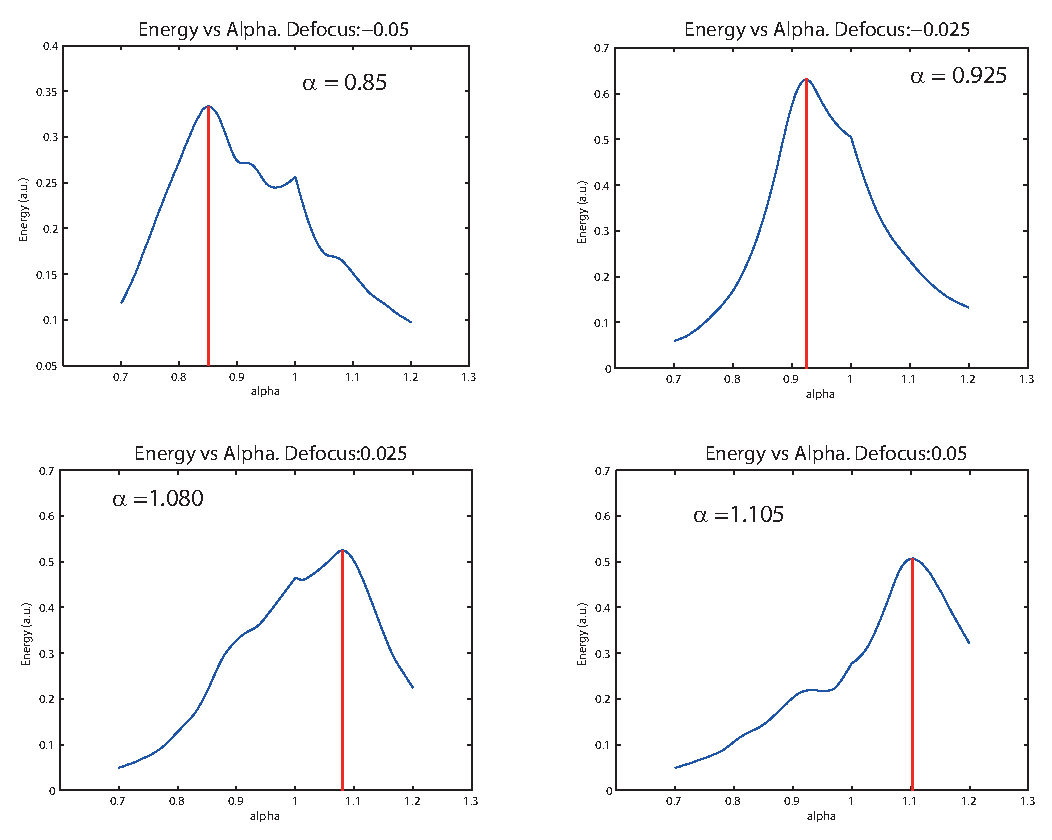
\includegraphics[width=1\textwidth]{C:/Users/Massimo/Documents/Thesis/Thesis_PhD/depthsp.eps}
 	\caption{\label{fig:maxima} Energy contained in the spectrum of the rendered image plotted as a function of the refocusing factor $ \alpha'$. In red is indicated the value of $ \alpha'$ corresponding to the image with the maximum energy. }
 \end{figure}
\begin{figure}[H]
	\centering
	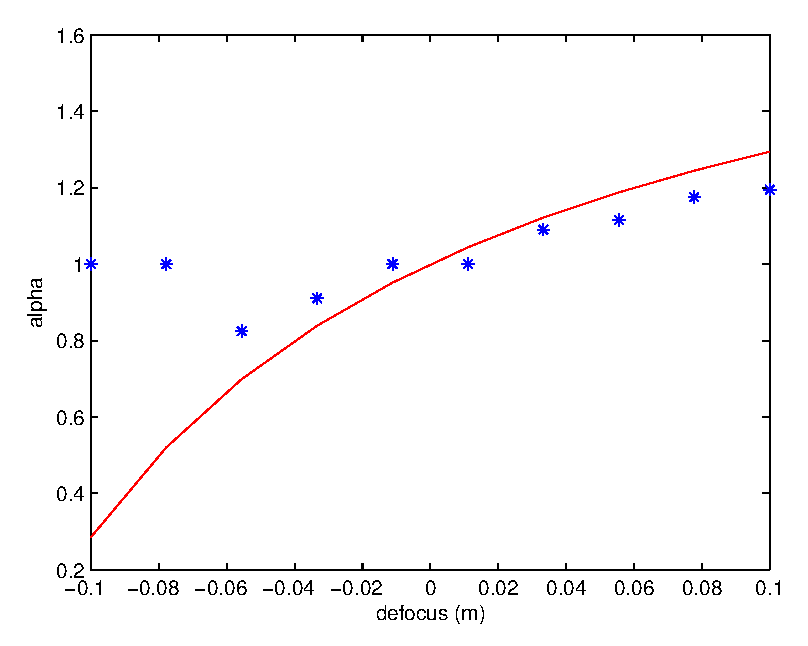
\includegraphics[width=.7\textwidth]{C:/Users/Massimo/Documents/Thesis/Thesis_PhD/errors1.eps}
	\caption{\label{fig:error} Estimated values of $ \alpha'$ represented by blue stars and the theoretical values represented with the red line. }
\end{figure}
\begin{figure}[H]
	\centering
	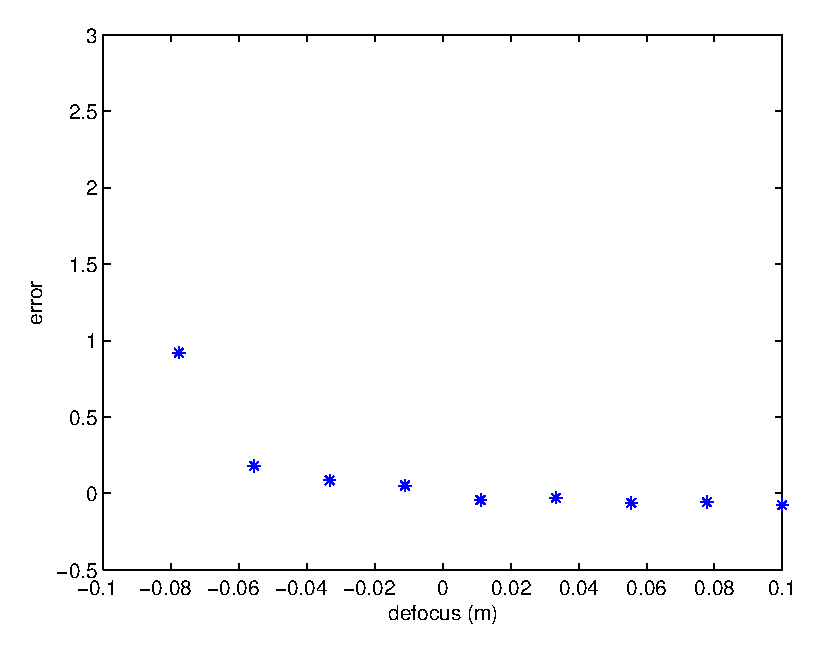
\includegraphics[width=.7\textwidth]{C:/Users/Massimo/Documents/Thesis/Thesis_PhD/errors2.eps}
	\caption{\label{fig:error1} Distance between the estimated values of $ \alpha'$ and the actual theoretical values. }
\end{figure}
The great difference between the theoretical and the estimated values of $\alpha'$ for defocus smaller than -0.02 m indicates that the method is not reliable when the object is too close to the main lens. Therefore those values should be discarded. This methods represents a proff of concept for a more elaborate development in a future work. It only works with point sources.
\section{Conclusions}
This chapter showed the results obtained simulating a plenoptic 1.0 imaging system using the Fresnel simulation toolbox described in chapter \ref{chap:fresnel}. With these simulation has been possible to evaluate for the first time the effects of diffarctions on the final image. An important result of this chapter is that the post processing algorithms obtained from ray optics theoretical models can be used to process raw images generated with a wave optics approach. This wave optics approach also led to the evaluation of the effects of diffraction on a plenoptic 1.0 system. A lenslet can be considered as a circular aperture whose diffraction pattern os the well known airy disk. If the fringes of the diffraction pattern of a lenslet extend on the neighbouring lenslet, cross-talk arise. To avoid the minimum diameter of a lenslet as indicated in equation \ref{eq:min_diam}.\\
The next step was to apply the rendering algorithm based on ray optics considerations already presented in literature and apply them on the raw images obtained from the wave optics simulations. All these methods gave the expected results proving that the simulation toolbox is capable to procuce realistic data. Particular attention was given to the depth estimation algorithm. With the help of the simulations it was possible to better understand and verify how the depth of an object can be estimated looking at the phase space. For a point source in focus the phase space look like a vertical straight line. if the point source is closer to the main lens the phase space will have a negative slope, while if it is further away from the main lens it will have a positive slope. This results perfectly match the theory. The synthetic refocus algorithm was also extensively analysed. Although this is not an original contribution to the field, it has been used to develop an original depth estimation method based on the creation of a focal stack of a point source refocused at different depth. It consist in refocusing the image of a point source at different depths and evaluate its power spectrum. The depth of the focal plane whose spectrum has the minimum energy will be value that better approximate the actual depth of the point source.\\
In coclusion, this chapter represents a link between the ray optics theoretical analysis of plenoptic imaging system extensively present in literature and its extension to wave optics. 
\nomenclature{$d_{Airy}$}{Airy disk diameter}
\nomenclature{$A'$}{Synthetic aperture}
\nomenclature{$ \alpha'$}{Refocusing factor}
\nomenclature{$F$}{Main lens - micro array distance}
\nomenclature{$F'$}{Main lens - synthetic focal plane distance}
\nomenclature{p}{Micro array pitch}
\nomenclature{$\delta\theta$}{Angular resolution}
\nomenclature{$N_{sub}$}{Sub-image resolution}
